\chapter{1T' $WSe_2$}

\section{Introduction}

The 1T and 1T' phases of group VI TMDCs have only recently gained significant attention compared to the more popular semiconducting 2H and number of reports in the literature has increased. They have been found to show promise in areas of electrocatalytic water splitting and energy storage thanks to lower charge transfer resistance \cite{Voiry2013}, a result of their metallic nature \cite{Wypych1992}. The 1T' phase is also predicted to be a large gap quantum spin Hall (QSH) insulator which can be useful in spintronic devices  application \cite{Chen2018}. In contrast to 1T' $WTe_2$ \cite{Fei2017} it can be used in ambient temperatures as well as ambient atmosphere unlike other known large gap QSH insulator materials like stanene \cite{Xu2013} or 2D In-Sb compounds \cite{Gruznev2018}. 

So far the synthesis of 1T and 1T' group VI sulfides and selenides ($MoS_2$, $WS_2$, $MoSe_2$, $WSe_2$)  phases has proven difficult due to the metastable nature of them. Most commonly a direct synthesis via e.g. a CVD route results in more thermodynamically stable 2H phase. The difference in energy per formula unit between 1H and 1T' $WSe_2$ phase is only 0.27 eV which suggests that under certain reaction conditions a metastable 1T' can be synthesised.

The $WSe_2$ flakes of varying thickness has been successfully grown via the colloidal synthesis method.

\section{Results}

In order to ascertain the phase of the as grown $WSe_2$ a Raman spectrum has been taken. As seen in Figure \ref{fig:1T'RamanSpectraComparison} the spectrum of the as grown 1T' $WSe_2$ looks very different to the Raman spectrum of the CVD grown 2H $WSe_2$ as seen in e.g. Figure \ref{fig:WSe2RamanSpectrum}. The $E^1_{2g}$ and $A_{1g}$ located around 250 $cm^{-1}$ and are convoluted in case of the monolayer. In spectrum of the 1T' sample (Figure \ref{fig:1T'RamanSpectraComparison}) the closest peaks to those are located at 248.6 and 260 $cm^{-1}$ and can be therefore ascribed to $E^1_{2g}$ and $A_{1g}$ modes respectively. Additionally the absence of the $B^1_{2g}$ peak suggest that the material is very thin. Furthermore there are 5 more unresolved peaks at 104.5, 149, 177, 218 and 236.3 $cm^{-1}$. Thus far there is no published information regarding the vibrational modes of 1T' $WSe_2$ and therefore the peaks cannot be assigned to the modes. Similarly new peaks have been reported for 1T' $MoS_2$ where new peaks were labelled as $J_1$, $J_2$ and $J_3$ \cite{Yu2018}.

\begin{figure}[!h]
	\begin{center}
		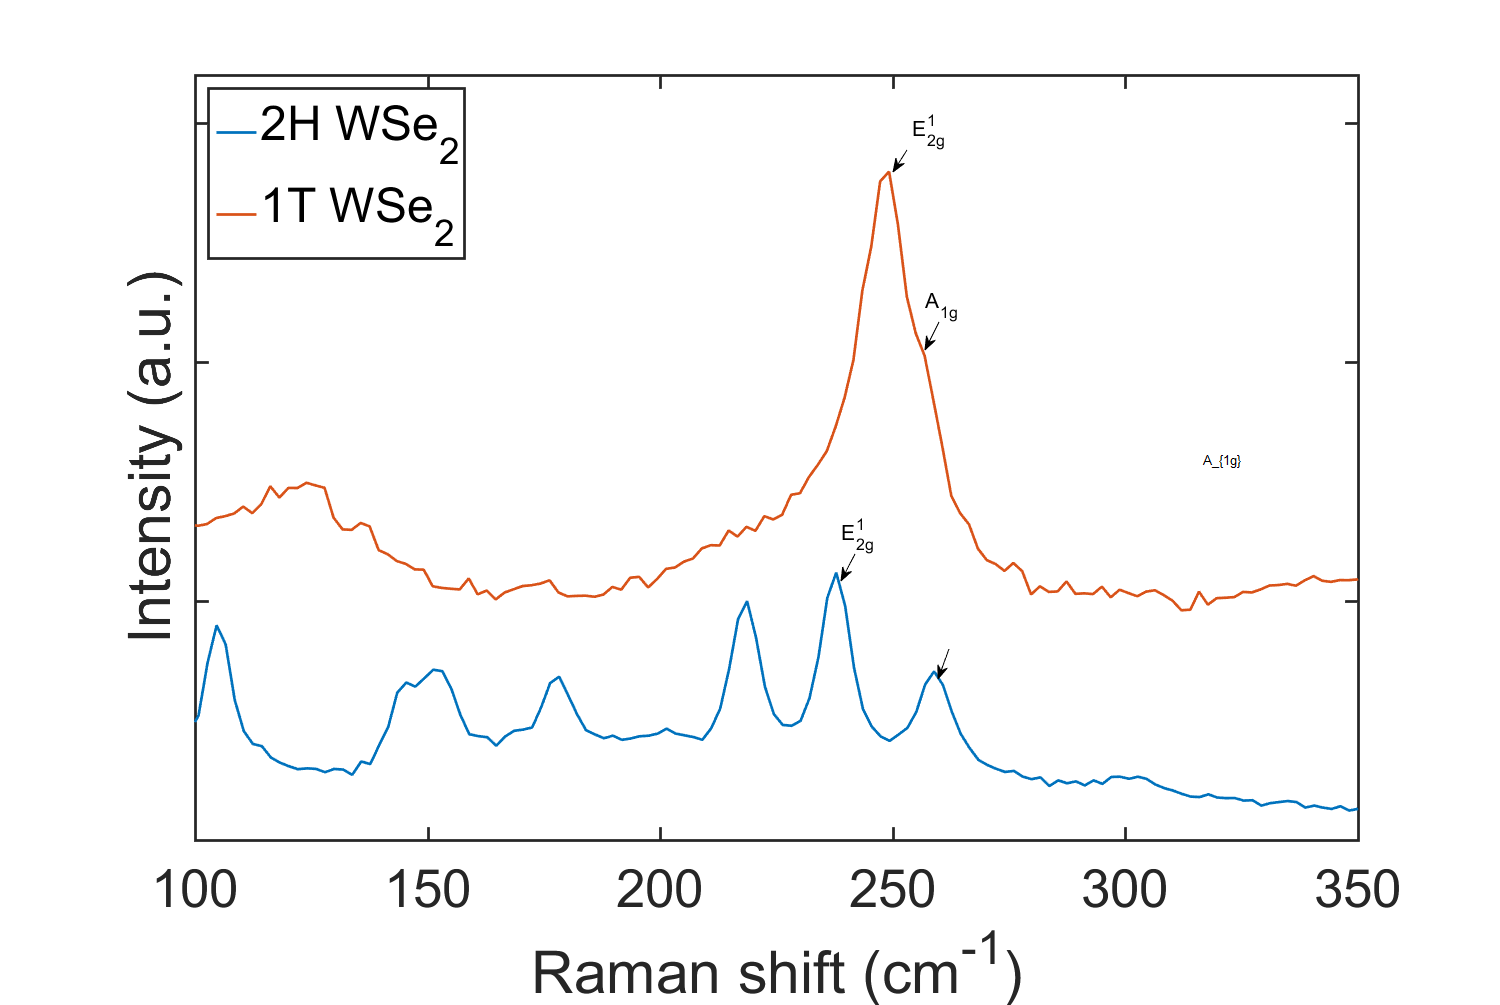
\includegraphics[scale=0.3]{1T'/RamanSpectraComparison.png}
		\caption{Raman spectra of 2H $WSe_2$ and 1T' $WSe_2$}
		\label{fig:1T'RamanSpectraComparison}
	\end{center}
\end{figure}

Similarly the XPS spectra were taken of the as-grown sample as seen in Figure \ref{fig:1T'XPSW4fPreSpectrum} and Figure \ref{fig:1T'XPSSe3dPreSpectrum}. The XPS spectrum of the W 4f electron shell shows a doublet of $W^{+4}$ 4f at 31.49 and 33.63 eV. This position varies notably from those reported for 2H $WSe_2$ and therefore are attributed to 1T' $WSe_2$. The shift itself is most likely caused by change in coordination of the metal atom or a change in the W-Se bond length from 2.531 \r{A} to 2.66 \r{A}. On top of the 1T' phase of $WSe_2$ additional small contributions to the spectrum can be attributed to the 2H $WSe_2$ at 32.22 eV and 34.30 eV. Additionally an even smaller contribution from tungsten oxides can be identified at 35.74 eV and 37.92 eV. The Se 3d level spectrum seen in Figure \ref{fig:1T'XPSSe3dPreSpectrum} of the as-grown sample has been fitted with 4 doublets. 2 of those doublets are associated with $Se^{-2}$ atoms and are assigned to 1T' $WSe_2$ (53.60 eV and 54.46 eV) and 2H $WSe_2$ (54.63 eV and 55.49 eV).

\begin{figure}[!h]
	\begin{center}
		\begin{subfigure}[b]{1\textwidth}
			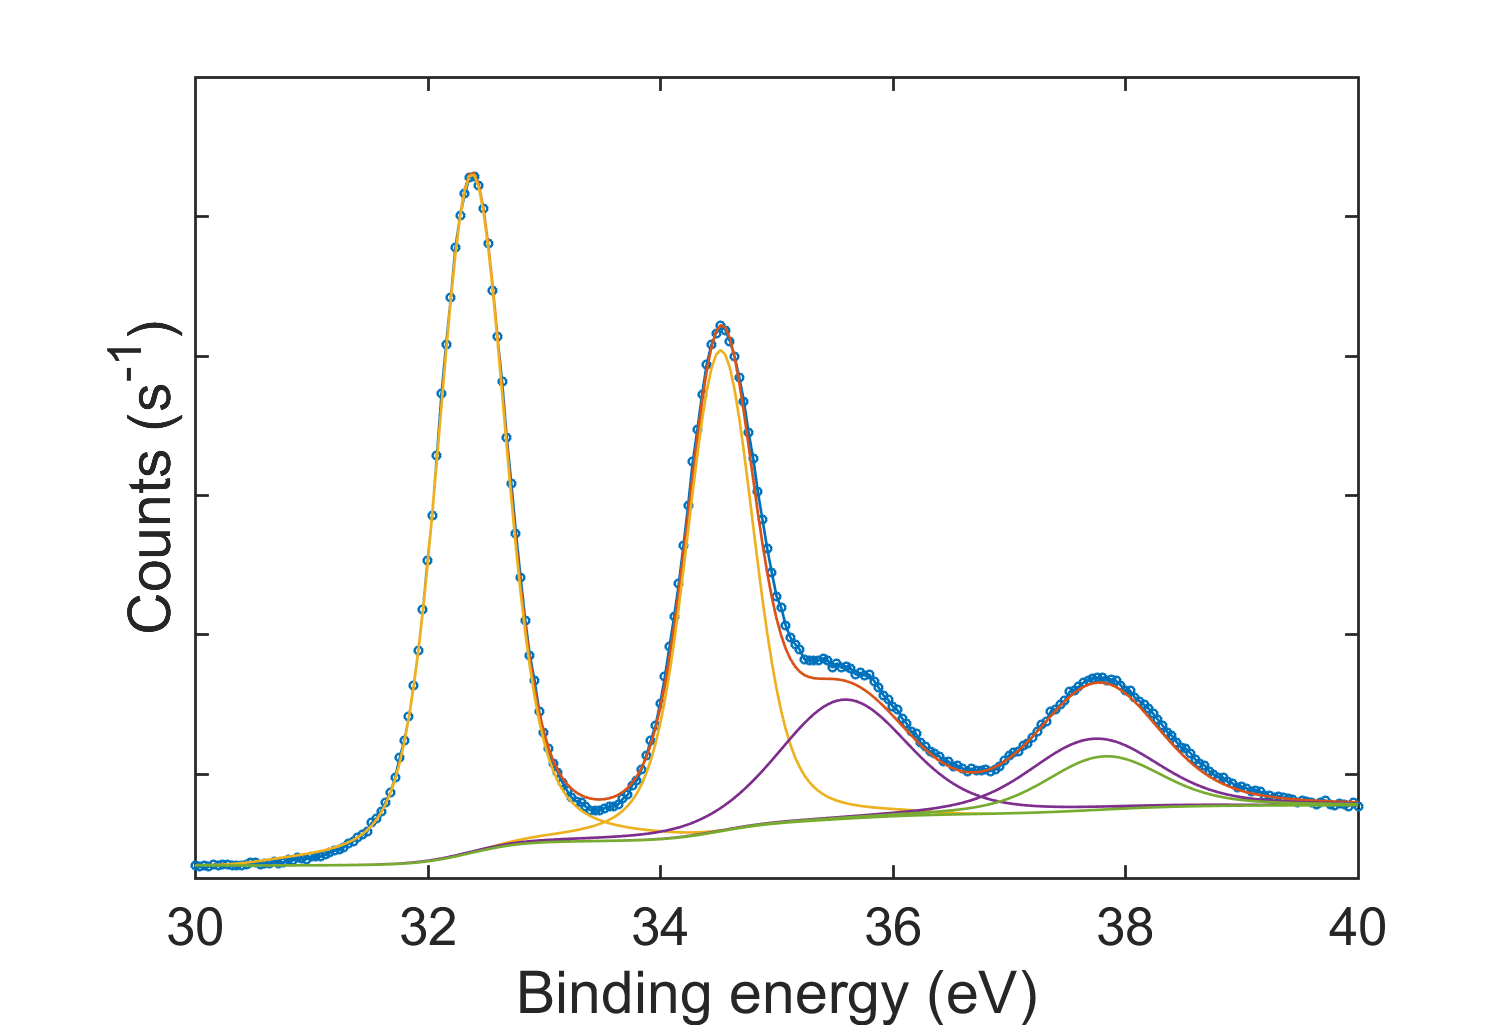
\includegraphics[scale=0.35]{1T'/XPSW4fPre.png}
			\caption{W 4f}
			\label{fig:1T'XPSW4fPreSpectrum}
		\end{subfigure}
		\qquad
		\begin{subfigure}[b]{1\textwidth}
			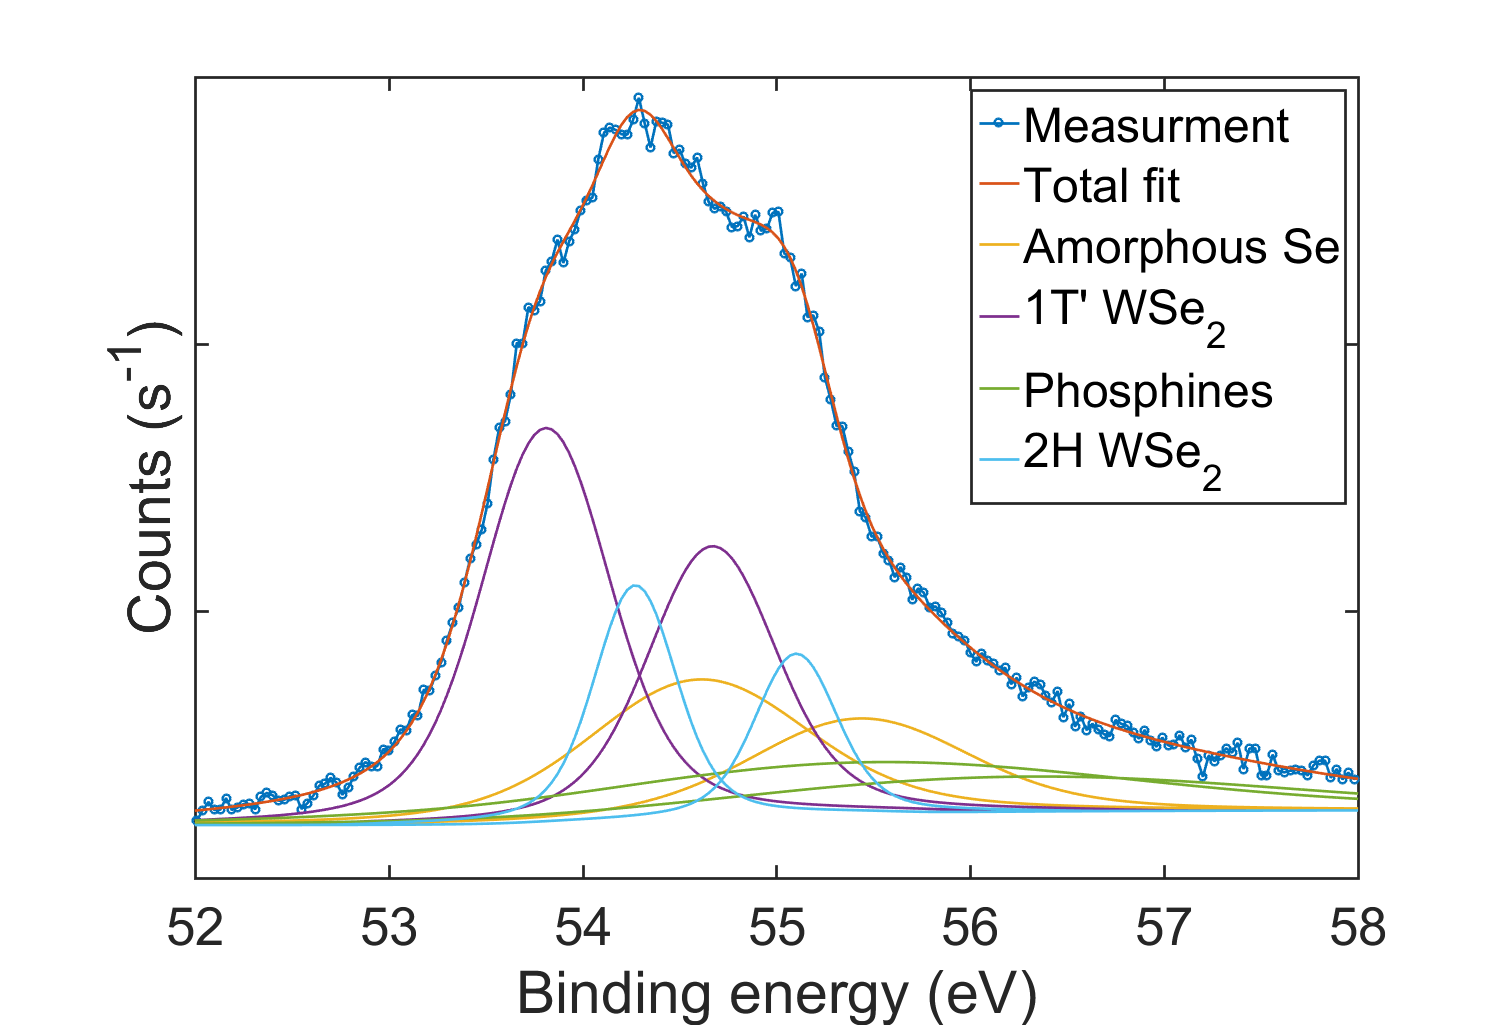
\includegraphics[scale=0.35]{1T'/XPSSe3dPre.png}
			\caption{Se 3d}
			\label{fig:1T'XPSSe3dPreSpectrum}
		\end{subfigure}
		\caption{XPS spectra of W 4f and Se 3d levels in as grown sample of $WSe_2$}
		\label{fig:1T'XPSPreSpectra}
	\end{center}
\end{figure}

\begin{figure}[!h]
	\begin{center}
		\begin{subfigure}[b]{1\textwidth}
			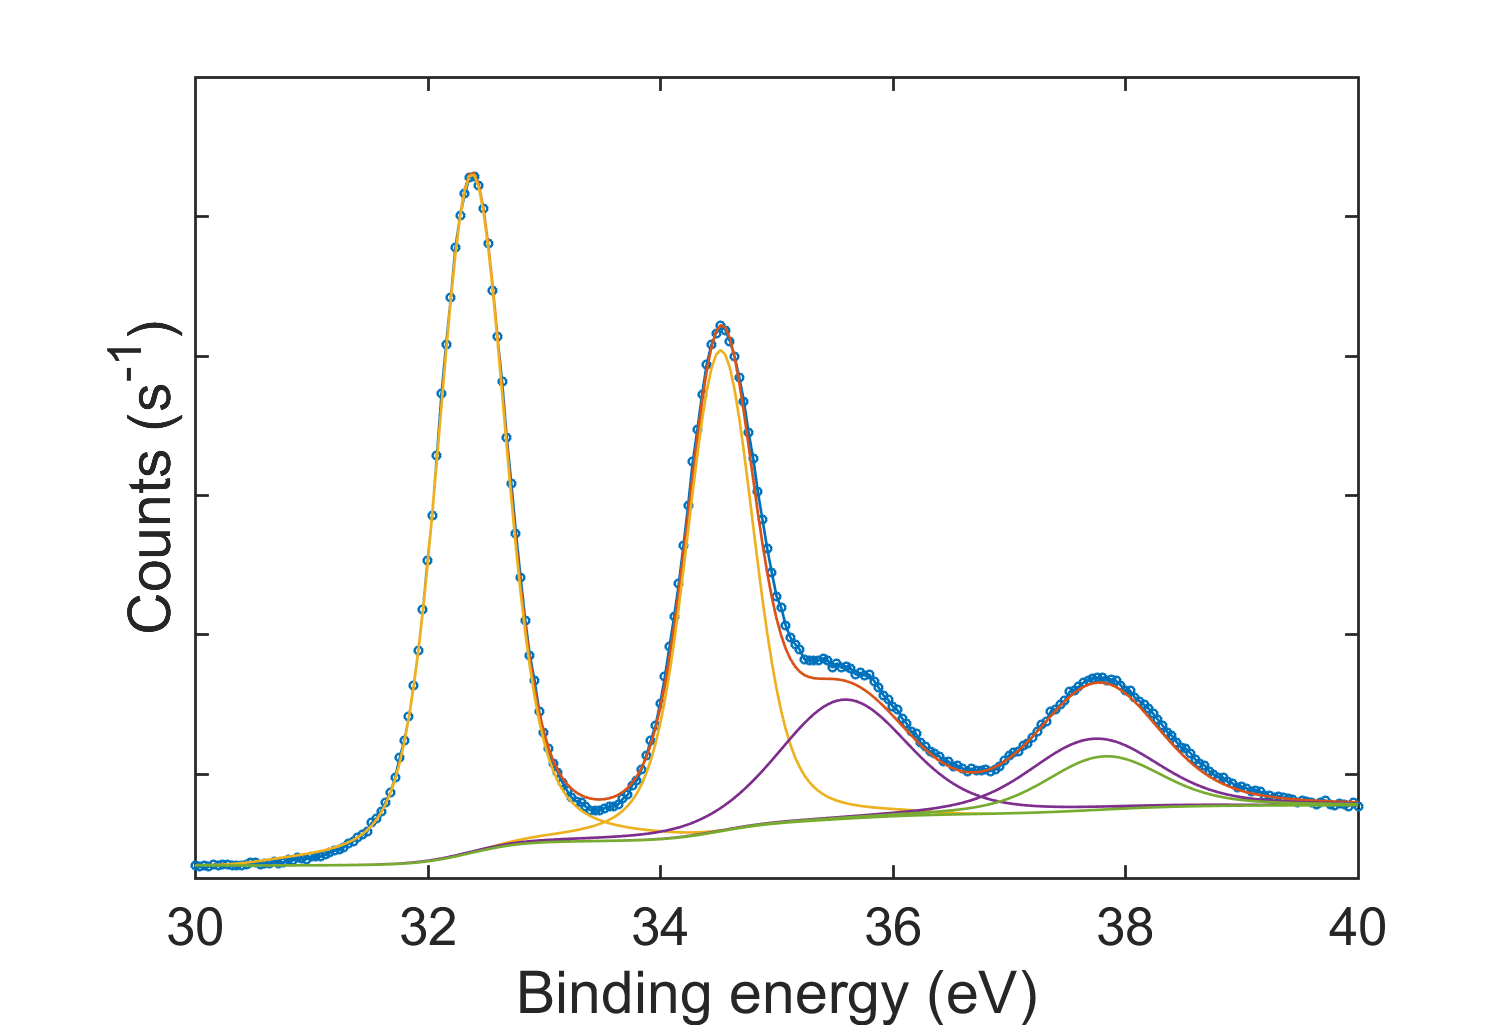
\includegraphics[scale=0.35]{1T'/XPSW4fAnn.png}
			\caption{W 4f}
			\label{fig:1T'XPSW4fAnnSpectrum}
		\end{subfigure}
		\qquad
		\begin{subfigure}[b]{1\textwidth}
			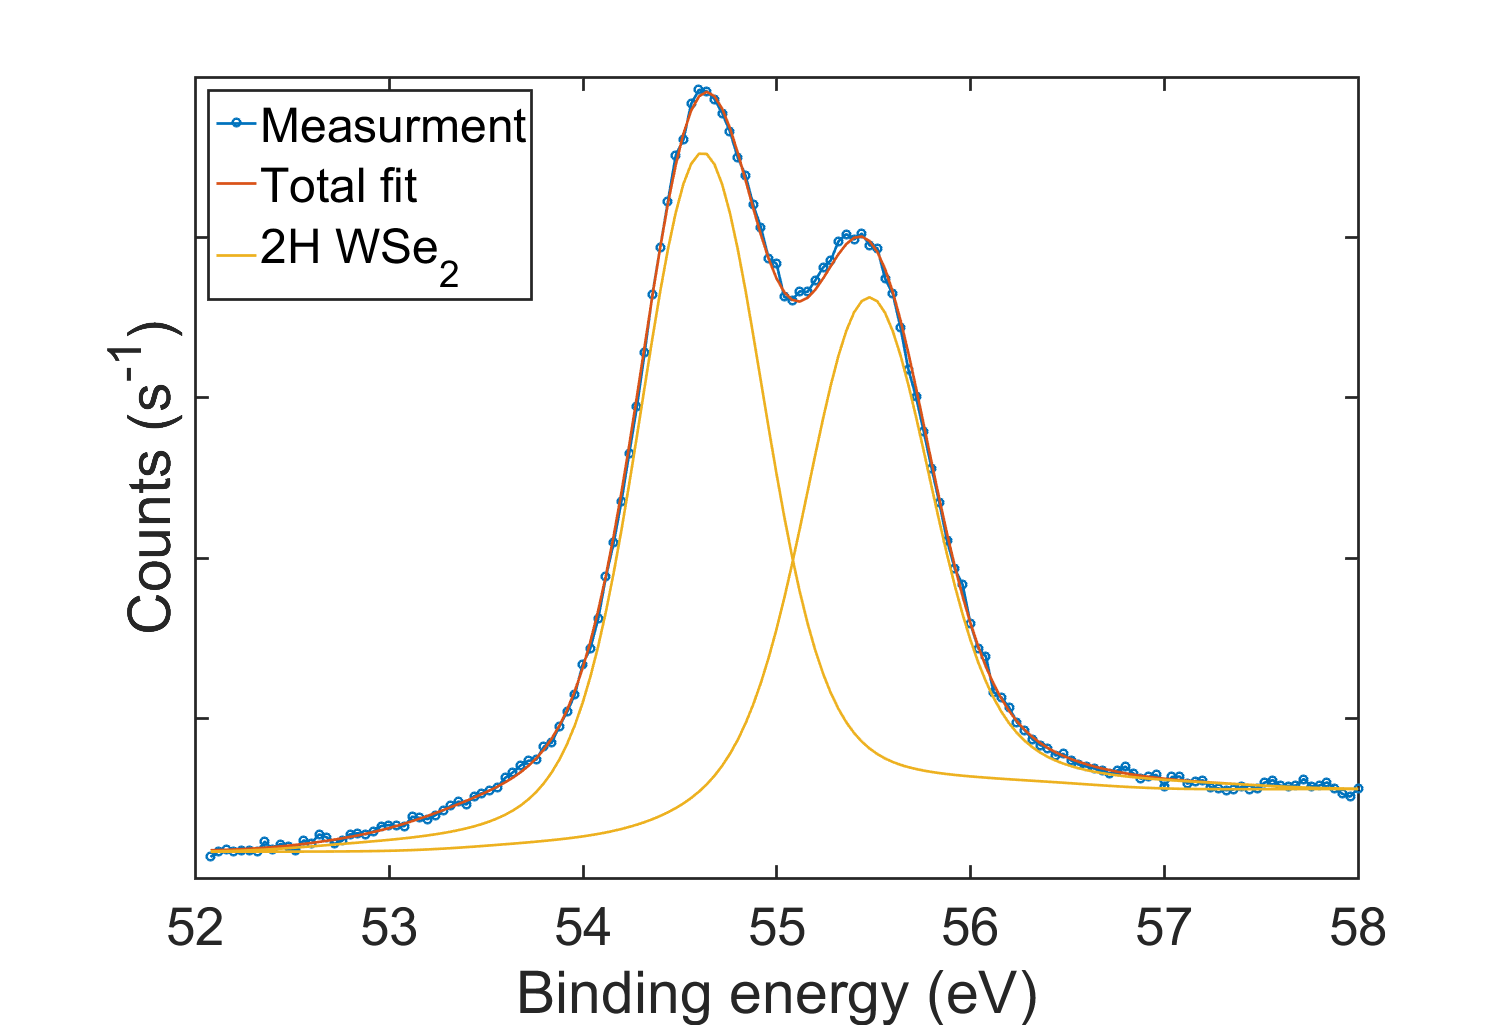
\includegraphics[scale=0.35]{1T'/XPSSe3dAnn.png}
			\caption{Se 3d}
			\label{fig:1T'XPSSe3dAnnSpectrum}
		\end{subfigure}
		\caption{XPS spectra of W 4f and Se 3d levels in the annealed sample of $WSe_2$}
		\label{fig:1T'XPSAnnSpectra}
	\end{center}
\end{figure}

The as-grown sample was then annealed at 400 {\degree}C in an argon atmosphere. The Raman spectrum of the annealed sample can be seen in Figure \ref{fig:1T'RamanSpectraComparison}. The previously unidentified peaks are no longer present except for the two convoluted peaks at around 250 $cm^{-1}$. This is indicative of 2H $WSe_2$ and suggests that the entirety of the 1T' phase has been converted to the 2H phase. Additionally the XPS spectra of the annealed sample can be seen in Figure \ref{fig:1T'XPSAnnSpectra}. The presence 4f $W^{4+}$ peaks 32.40 eV and 34.58 eV and the almost complete absence of the 1T' 4f $WSe_2$ indicates that the sample is primarily a 2H $WSe_2$. Following the annealing the XPS spectrum of the Se 3d can be seen in Figure \ref{fig:1T'XPSSe3dAnnSpectrum}. The spectrum can be fitted with one doublet associated with 2H $WSe_2$.

The sample was also characterised using TEM as seen in Figure \ref{fig:1T'TEMMaps}. The TEM images show well defined flower shaped nanostructures with the average diameter of 200 nm. The petals stem from the central point and thin down towards the edges down to single layer. The single petals appear to be of 1T' phase while each petal is a single crystal. An experimentally acquired FFT patterns show kinematically forbidden (010) reflections which can indicate presence of antisite defects. Additionally the structural parameters $a = 5.76$ \r{A} and $b = 3.30$ \r{A} have been identified. The $a$ parameter is smaller than the calculated value of 5.94 \r{A} \cite{Duerloo2014} which can be attributed to the scrolling of the flexible petals along the [010] direction perpendicular to the petal rim.

\begin{figure}[!h]
	\begin{center}
		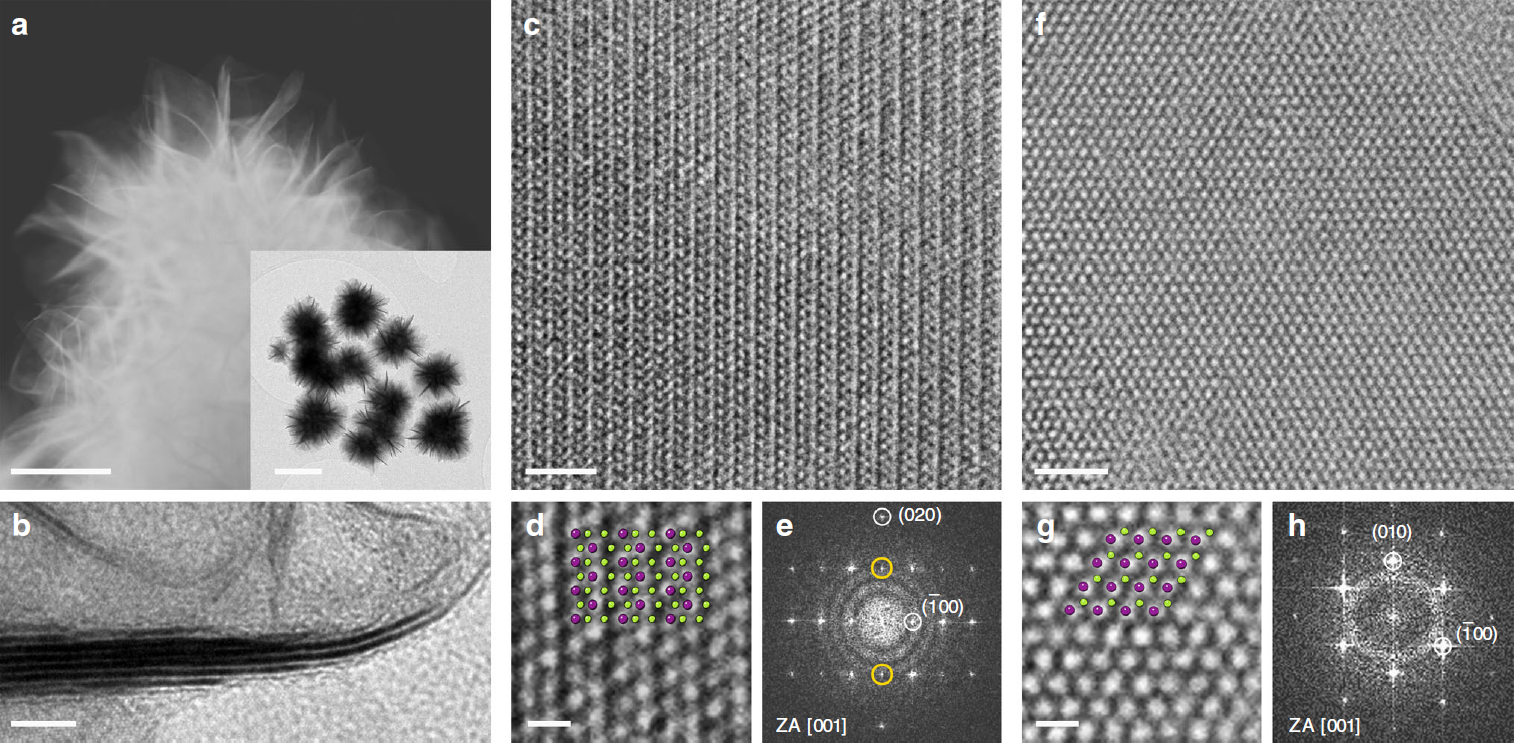
\includegraphics[scale=0.3]{1T'/TEMMaps.png}
		\caption{Transmission electron microscopy (TEM) characterisation of the colloidal $WSe_2$ nanostructures. a) Annular dark-field scanning TEM image of a $WSe_2$ branched nanoflower illustrating ultra-thin nature of individual nanosheets (scale bar: 100 nm), inset — an overview image of an ensemble of the $WSe_2$ nanoflowers (scale bar: 200 nm). b) Side view TEM image of an individual petal thinning down to monolayer at the rim (scale bar: 5 nm). c) High-resolution TEM image of the as-produced $WSe_2$ nanosheets demonstrating a continuous 1T’ phase over a large area (scale bar: 2 nm); d) zoomed in image (scale bar:
0.5 nm) with an overlaid crystal model of the 1T’ phase of $WSe_2$ illustrating the zigzag chains of tungsten atoms; e) fast Fourier transform (FFT) pattern of the area shown in c, yellow circles highlight kinematically forbidden (010) reflections. f) High-resolution TEM image of the annealed $WSe_2$ nanosheets (scale bar: 2 nm); g) zoomed in image (scale bar: 0.5 nm) with an overlaid crystal model of the 2H $WSe_2$ phase displays the uniformly spaced hexagonal lattice; h) FFT pattern of the area shown in f. In the overlaid crystal models, purple circles represent tungsten atoms, and green circles represent selenium atoms}
		\label{fig:1T'TEMMaps}
	\end{center}
\end{figure}

In order to investigate the samples electronic properties the Kelvin probe force macroscopy (KPFM) as seen in Figure \ref{fig:1T'ElectronicProperties}. The work function of the 2H and 1T' phase was calculated using the known values of work function for p-doped Si. The values were found to be 2.6 eV and 4.2 eV respectively and they were found to be in good agreement with the values of the 2H (4.08 eV) and 1T' (2.36 eV) produced by potassium surface functionalisation \cite{Lei2018}. 

\begin{figure}[!h]
	\begin{center}
		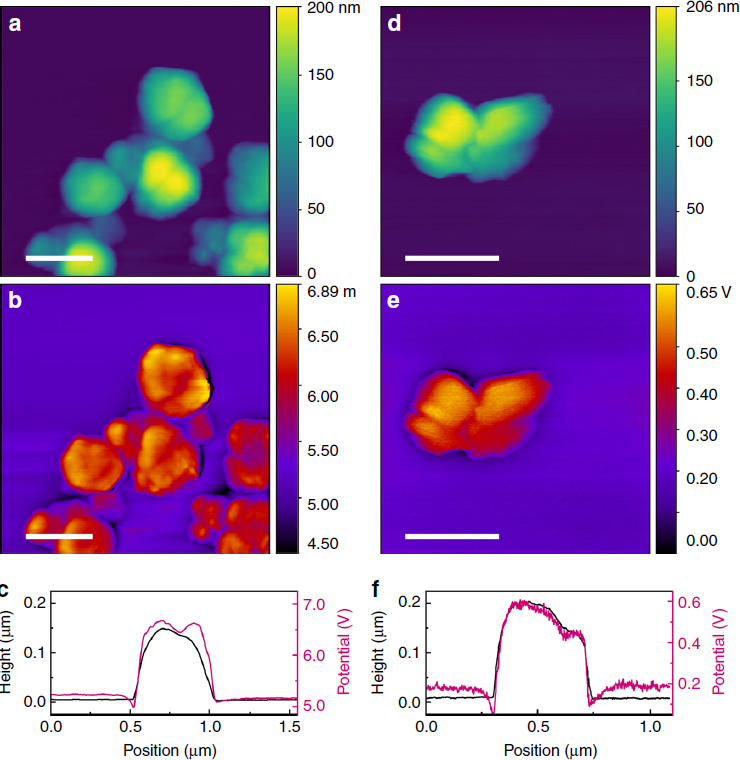
\includegraphics[scale=0.3]{1T'/ElectronicProperties.png}
		\caption{Electronic properties of the 1T’ and 2H $WSe_2$ nanosheets. a) Tapping mode atomic force microscopic (AFM) image, b) Kelvin probe force microscopic (KPFM) image and (c) height profile (black) and the corresponding contact potential difference variation (purple) of the as-produced 1T’ $WSe_2$ nanoflowers assembled on a p-doped Si wafer. d) Tapping mode AFM image, e) KPFM image and f) the line scans of the annealed 2H $WSe_2$ nanoflowers. Scale bars: 500 nm}
		\label{fig:1T'ElectronicProperties}
	\end{center}
\end{figure}

\section{Conclusions}

The 1T' $WSe_2$ has been grown via the colloidal synthesis route with flakes with average diameter of 200 nm. The sample has then been characterised using Raman spectroscopy, XPS, TEM, and KPFM. Following an annealing at 400 {\degree}C the 1T' phase has been almost entirely converted to 2H. This growth method allows therefore for direct deposition of metastable phase on a functional substrate. As a scalable process it shows promise for potential growth of other metastable phases of materials. 